\section{Efficient frontier}
\label{sec:frontier}

We compare the momentum allocation with mean-variance optima using all twenty
nonzero targets at first formation, February 27, 2026. Reference weights use
the original sizing NAV of \$1,000,767.40.

\subsection{Estimation and constraints}

We retain only months with returns for all twenty stocks. SNDK began trading
in February 2025 after separating from Western Digital \citep{wdc2025sandisk},
so our sixty-month lookback yields only twelve common monthly returns,
March 2025-February 2026. Requests for 12, 24 or 36 months yield the same sample.
February's month-end label represents the February 27 close. We compute adjacent-month returns before
removing incomplete intervals, without filling prices, bridging gaps or
stitching different securities.

Following \citet{markowitz1952}, annual arithmetic means and covariance are
\begin{equation}
 \widehat{\boldsymbol\mu}=12\bar{\mathbf r},
 \qquad
 \widehat{\boldsymbol\Sigma}
 =12\left[(1-\delta)S_{\mathrm{ML}}
 +\delta\frac{\operatorname{tr}(S_{\mathrm{ML}})}{20}I\right].
\end{equation}

Ledoit-Wolf shrinkage uses centered covariance normalized by $n$, a spherical
target and fitted $\delta=0.3095$ \citep{ledoitwolf2004,sklearncovariance}.
It raises covariance rank from eleven to twenty, with condition number 26.03.

Both feasible sets preserve stock directions and sleeve totals:
\begin{equation}
  \sum_{i\in\mathcal L}w_i=1.05,
  \qquad \sum_{i\in\mathcal S}w_i=-0.45.
\end{equation}

\emph{Bounded} weights stay between $0.5$ and $2$ times their original
magnitudes, retaining ten longs and ten shorts. \emph{Relaxed} weights can be
zero or reach their sleeve total, allowing portfolios below the competition's
position minimum. Neither set imposes sector neutrality.

We trace each efficient branch from its global minimum-variance portfolio
(GMV) using one hundred return targets, and separately maximize
\begin{equation}
 U(\mathbf w)=\mathbf w^{\mathsf T}\widehat{\boldsymbol\mu}
 -\frac{\lambda}{2}\mathbf w^{\mathsf T}\widehat{\boldsymbol\Sigma}\mathbf w,
 \qquad \lambda=2.8741.
\end{equation}

Indifference curves satisfy $\mu_p=U_0+\lambda\sigma_p^2/2$ in annual decimal
units. An independent linear certificate checks feasibility and the
first-order optimality gap.

\begin{figure}[H]
  \centering
  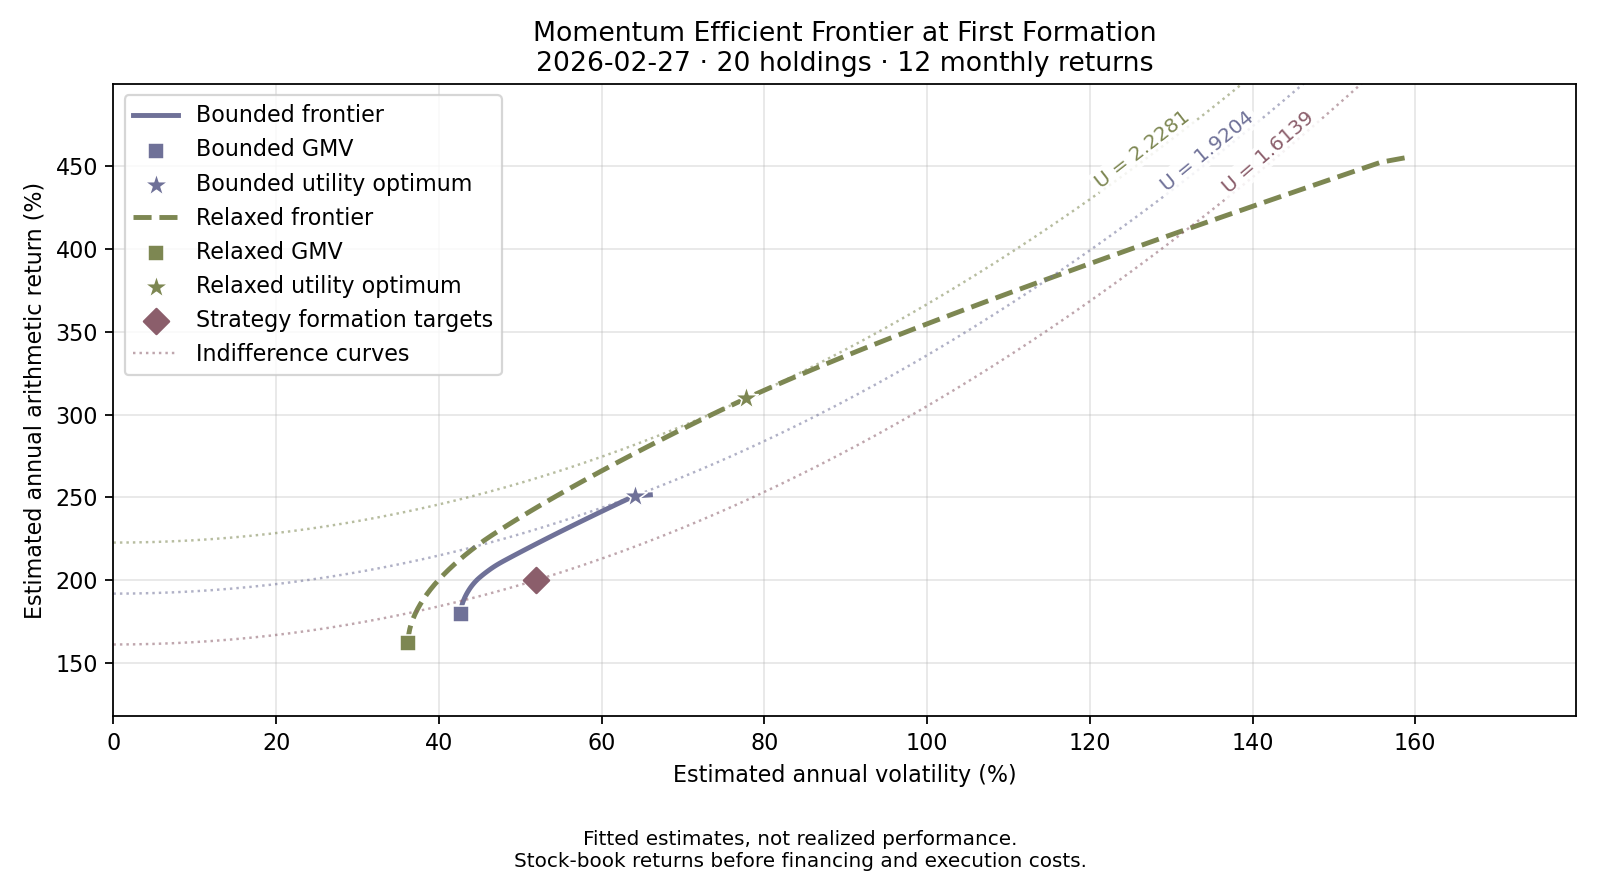
\includegraphics[width=\reportfigurewidth]{../outputs/efficient_frontier/momentum/figures/frontier.png}
  \caption[First-formation frontier and indifference curves]{First-formation frontier and indifference curves for all twenty
  targets.}
  \label{fig:frontier}
\end{figure}

\begin{samepage}
\subsection{Allocation and sensitivity}

At the formation portfolio's estimated return, bounded reallocation lowers
volatility from 51.99\% to 44.66\%; the relaxed minimum is 39.95\%.
Both bounded optima retain ten longs and ten shorts, with a 21\% largest
position. The relaxed GMV holds eight longs and four shorts, with a 25.41\%
largest position; GMV utilities are 1.538 bounded and 1.432 relaxed.
The relaxed utility optimum concentrates into three longs and two shorts,
with 43.02\% in the largest position.
\par
\end{samepage}

The large fitted returns reflect short-sample annualization and leverage.
The sample also overlaps parameter selection, so these are in-sample allocation
comparisons. \Cref{tab:frontier-sensitivity} tests estimation and constraint
choices.

\begin{table}[H]
  \centering
  \begin{threeparttable}
  \small
  \begin{tabularx}{\linewidth}{@{}X r r r@{}}
    \toprule
    Estimation or constraint case & Return (\%) & Vol. (\%) & Utility \\
    \midrule
    Primary Ledoit-Wolf & 251.16 & 64.14 & 1.920 \\
    Means shrunk 50\% & 121.89 & 47.70 & 0.892 \\
    20\% diagonal covariance shrinkage & 238.35 & 65.78 & 1.762 \\
    50\% diagonal covariance shrinkage & 248.25 & 62.05 & 1.929 \\
    Tighter bounds: $0.75$-$1.5\times$ & 225.68 & 57.81 & 1.776 \\
    Wider bounds: $0.25$-$3\times$ & 285.63 & 73.49 & 2.080 \\
    Leave one month out: range & 206.53-283.17 & 51.09-68.55 & 1.682-2.292 \\
    \bottomrule
  \end{tabularx}
  \caption[Sensitivity of the bounded utility optimum]{Sensitivity of the bounded utility optimum. Rows use the same primary sample except the explicitly labelled leave-one-month-out perturbations.}
  \label{tab:frontier-sensitivity}
  \end{threeparttable}
\end{table}

Mean shrinkage pulls each stock halfway toward the cross-sectional mean.
The diagonal cases use unbiased ($n-1$) sample covariance, unlike the primary
estimator's $n$ normalization and spherical target; both features therefore
change. Leave-one-month-out ranges are perturbations, not confidence
intervals. Shrinkage improves conditioning, but expected returns remain poorly
estimated.
\FloatBarrier
